\documentclass[]{IEEEtran}
% some very useful LaTeX packages include:
%\usepackage{cite}      
\usepackage{graphicx}   
\usepackage{subfigure} 
\usepackage{url}       
\usepackage{amsmath}    
\usepackage{caption2}
% Your document starts here!
\begin{document}

% Define document title and author
	\title{Weekly Report}
	\author{Adviser: Prof. Yang Wen \\Student: Cheng Wensheng\\ Period: 2018.9.16-9.23
	}
	\markboth{Visual Information Processing Group}{}
	\maketitle

% Write abstract here
\begin{abstract}
	This week I mainly put my effort on reviewing the paper and writing project application plan.
\end{abstract}

% Each section begins with a \section{title} command
\section{Sar contest}
	% \PARstart{}{} creates a tall first letter for this first paragraph
	\PARstart{T}{he} final result of the SAR image processing contest came out. Guo Wei and Lei Xu took part in the conference and let us know more information.
	\begin{itemize}
		\item The situation of the SAR image building extraction is so competitive and close. The first 3 teams all got 62\% F1 score. The difference is so small.
		\item Although we got 4th in this contest, the best result of our history grades can ranked 2nd in the final result. Since some rules are not so clear in this competition, such as the grades are not public and the test set changed, we may change our strategy and keep our grades.
		    
	\end{itemize}
	
	

\section{Project plan}
% \PARstart{}{} creates a tall first letter for this first paragraph
\PARstart{F}{or} the equipment and education department project, we finished the whole file work, mainly assisting Yu Huai and Xu Fang.
\begin{itemize}
	\item I was in charge of the ordinary image to SAR image transformation part. The topic of the whole work is detecting and interpreting with RGB and registered SAR image, and this part is to generate many SAR images artificially, since it's hard to get lots of SAR images.
	\item This part is based on cGAN and the classic work of image-to-image translation. Its input are RGB images and their registered images. The generator generates SAR-like images with features of both RGB iamge and SAR image. The discriminator decides whether the SAR-like image is true enough. Finally we can use this network to generate SAR image with RGB image as input, which is useful for following procedures. 
	
\end{itemize}

Fig.~\ref{fig:fw} is the cGAN model. Fig.~\ref{fig:rt} is the network pipeline.

\newpage


\begin{figure}
	\vspace{0.5cm}
%	\begin{minipage}[t]{0.5\linewidth}
		\centering
		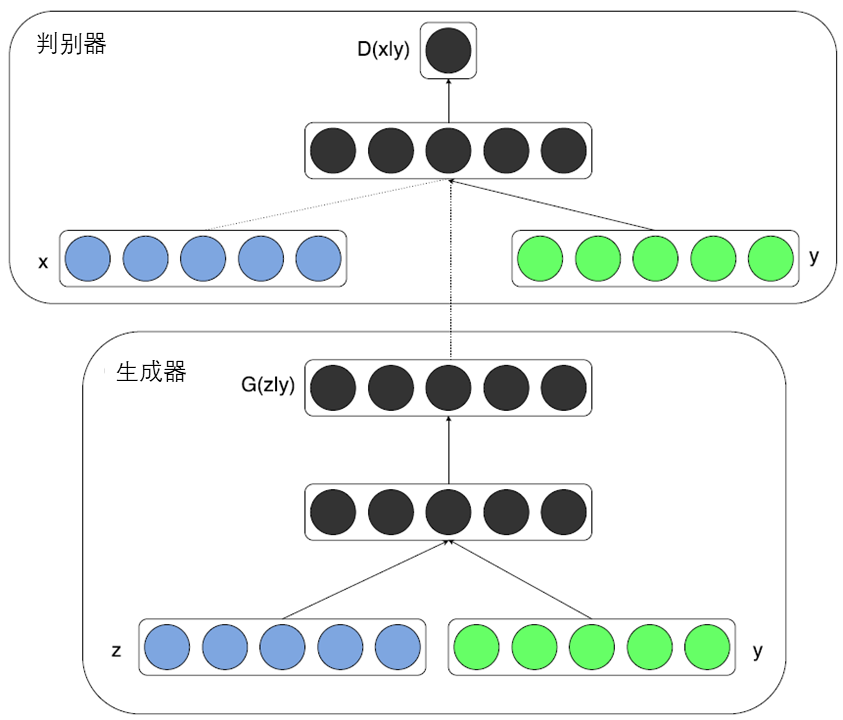
\includegraphics[width=0.7\columnwidth]{fw}
		\caption{cGAN model}
		\label{fig:fw}
%	\end{minipage}%
%	\begin{minipage}[t]{0.5\linewidth}
	\vspace{0.3cm}
		\centering
		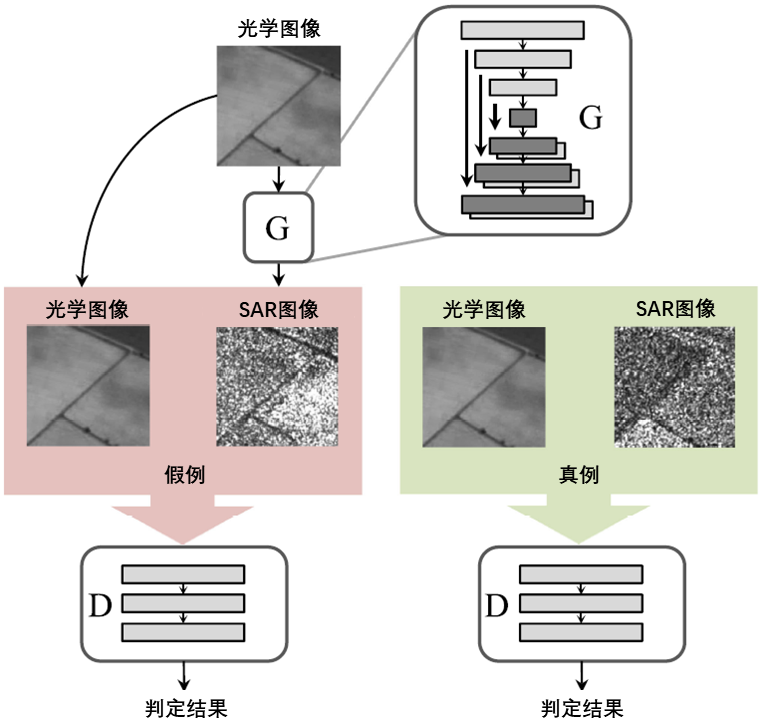
\includegraphics[width=0.7\columnwidth]{rt}
		\caption{Network pipeline}
		\label{fig:rt}
%	\end{minipage}
\end{figure}


%\begin{figure}[!hbt]
%%		 Center the figure.
%		\vspace{0.7cm}
%%		\hspace{50cm}
%		\begin{center}
%			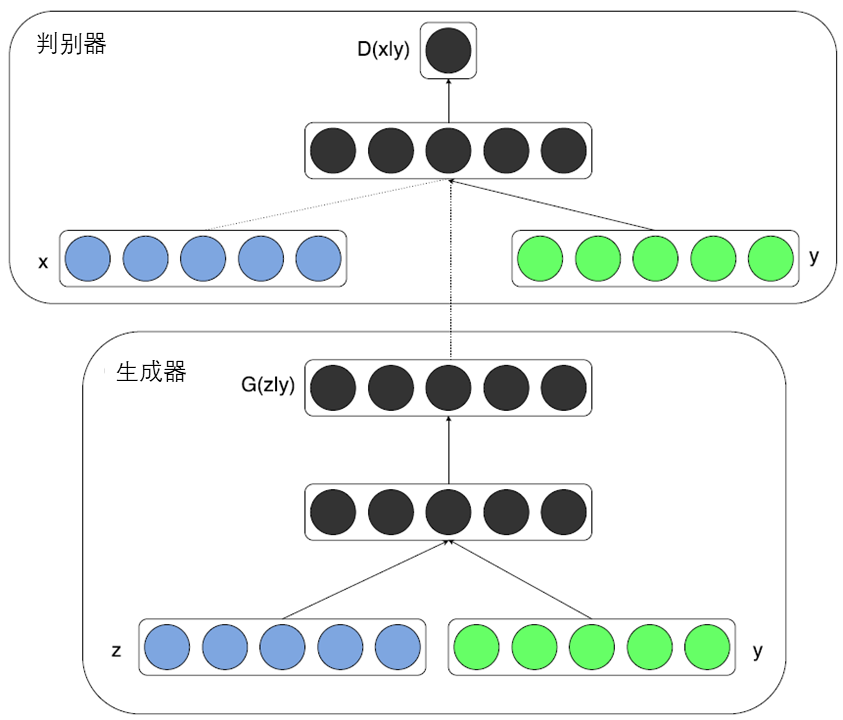
\includegraphics[width=0.2\columnwidth]{fw}
%				%		 Create a subtitle for the figure.
%			\caption{CNN methods result}
%			\label{fig:fw}
%		    \vspace{0.2cm}
%			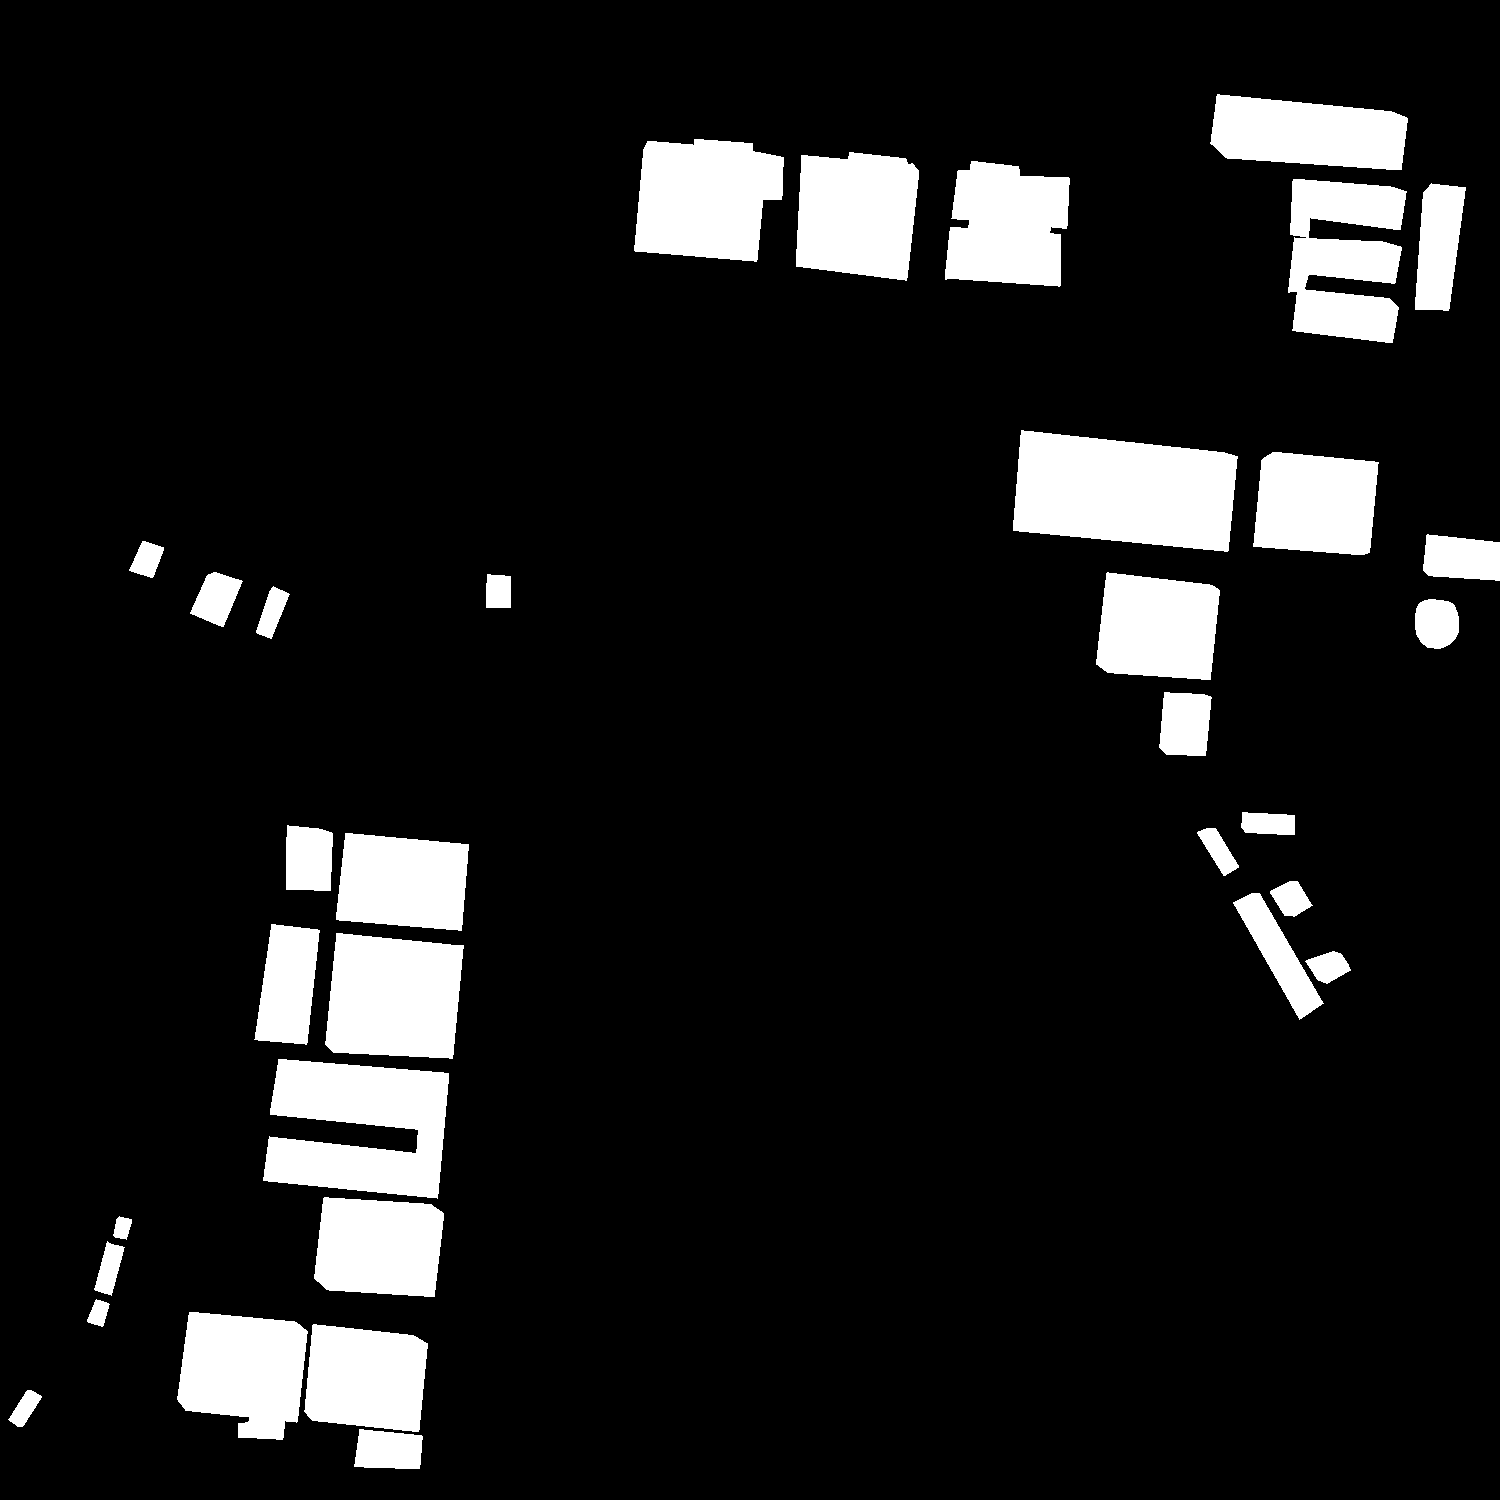
\includegraphics[width=0.2\columnwidth]{rs}
%				%Create a subtitle for the figure.
%			\caption{Ground truth}
%			\label{fig:rt}
%		\end{center}
%	\end{figure}



% Your document ends here!
\end{document}